\documentclass{beamer}
\usetheme{Madrid}
\usepackage{pifont}
\usepackage{amsmath}
\usepackage{geometry} 
\usepackage{svg}
\usepackage{graphicx}
\usepackage{tikz}

\graphicspath{ {./assets/} }
\usetikzlibrary{positioning}



\title{Adaptasi Positional Encoding pada Arsitektur Transformer untuk Sintesis Notasi Gamelan yang Koheren dan Terkendali}
\author{Arif Akbarul Huda}

\begin{document}
	\begin{frame}
		\titlepage
	\end{frame}
	
	\begin{frame}
		\frametitle{Previous Work}
		\framesubtitle{Plotting Structure}
		\begin{columns}
			
			% --- First Column (Left Image) srepeg-tlutur-sl-sanga.png---
			\begin{column}{0.5\textwidth}
				\begin{figure}
					\centering
					\includegraphics[width=1 \linewidth]{srepeg-tlutur-sl-sanga.png}
					\caption{Notasi Gamelan}			
				\end{figure}		
			\end{column}
			
			% --- Second Column (Right Image) ---
			\begin{column}{0.5\textwidth}
				\begin{figure}
					\centering
					\includegraphics[width=1 \linewidth]{plot-struktur-gamelan.png}
					\caption{Plot Struktur}			
				\end{figure}		
			\end{column}
		\end{columns}
	\end{frame}

	\begin{frame}
		\frametitle{Insight}
		\begin{figure}
			\centering
			\includegraphics[height=0.5 \linewidth]{book-fundamental-music-processing.png}
			\caption{Buku Referensi}			
		\end{figure}
	\end{frame}

	\begin{frame}
		\frametitle{Insight}
		\framesubtitle{Chapter 4. Music Structure Analysis}
		\begin{columns}
			
			% --- First Column (Left Image) srepeg-tlutur-sl-sanga.png--- structural-analysis.png
			\begin{column}{0.5 \textwidth}
				\begin{figure}
					\centering
					\includegraphics[width=1 \linewidth]{structural-analysis.png}
					\caption{4.1. From the book}
				\end{figure}
			\end{column}
			
			% --- Second Column (Right Image) ---
			\begin{column}{0.5 \textwidth}
				The General Goal of Music Structural Analysis
				\begin{itemize}
					\item  Temporal Segmentation
					\item  Structural Identification
					\item  Categorical Grouping
				\end{itemize}
				The methods
				\begin{itemize}
					\item  Repition-based
					\item  Novelty-based
					\item  Homogeneity-based
				\end{itemize}
				
			\end{column}
		\end{columns}
	\end{frame}
	\begin{frame}
		\frametitle{Insight}
		\framesubtitle{Chapter 4. Music Structure Analysis}
		\begin{columns}
			
			% --- First Column (Left Image) srepeg-tlutur-sl-sanga.png--- structural-analysis.png
			\begin{column}{0.5 \textwidth}
				\begin{figure}
					\centering
					\includegraphics[width=1 \linewidth]{structure-annotatoins-labeling-evaluation.png}
					\caption{4.30. From the book}
				\end{figure}
			\end{column}
			
			% --- Second Column (Right Image) ---
			\begin{column}{0.5 \textwidth}
				Evaluation
				\begin{itemize}
					\item  Precision, Recall, F-Measure
					\item  Structure Annotations
					\item  Labeling Eval.
					\item  Boundary Eval.
					\item  Thumbnail Eval.
				\end{itemize}
				
			\end{column}
		\end{columns}
	\end{frame}
	\begin{frame}
		\frametitle{Insight}
		
		
		Subjective evaluation are
		\begin{itemize}
			\item  Unscalable
			\item  Inability to Guide Improvement
			\item  Missing the "Why"
		\end{itemize}
	 	\vspace{1cm}
		\tiny de Berardinis, J., Cangelosi, A. and Coutinho, E. (2022) “Measuring the Structural Complexity of Music: From Structural Segmentations to the Automatic Evaluation of Models for Music Generation,” IEEE/ACM Transactions on Audio, Speech, and Language Processing, 30, pp. 1963–1976. Available at: https://doi.org/10.1109/TASLP.2022.3178203.
	\end{frame}

	
	
	\begin{frame}
		\frametitle{Insight}
		\begin{figure}
			\centering
			\includegraphics[height=0.5 \linewidth]{interval-in-cent.png}
			\caption{Struktur interval dalam cent antara slendro, pelog dan western}			
		\end{figure}
	\end{frame}

	\begin{frame}
		\frametitle{Insight}
		\begin{figure}
			\centering
			\includegraphics[height=0.5 \linewidth]{bunyi-overtone-harmoni.png}
			\caption{Kempul nada 6}			
		\end{figure}
	\end{frame}

	\begin{frame}
		\frametitle{Insight}
		\framesubtitle{Kenong pada laras slendro}

		% Begin the columns environment
		\begin{columns}
			
			% --- First Column (Left Image) ---
			\begin{column}{0.5\textwidth}	
				\begin{center}
					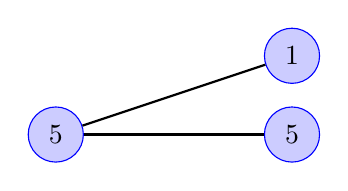
\begin{tikzpicture}[
						% Define a style for all nodes (optional, but helpful)
						node style/.style={circle, draw=blue, fill=blue!20, minimum size=7mm}
						]
						
						% Define and place your nodes
						\node[node style] (A) at (0, 0) {5};
						\node[node style] (B) at (3, 1) {1};
						\node[node style] (C) at (3, 0) {5};
						
						% --- Draw the edges ---
						\draw[thick] (A) -- (B); 
						\draw[thick] (A) -- (C); 
					\end{tikzpicture}
					\vspace{12pt}
					\par %
					{Kenong nada 5 digunakan untuk me-ngenongi nada 1 dan 5}
				\end{center}	
			\end{column}
			
			% --- Second Column (Right Image) ---
			\begin{column}{0.5\textwidth}
				\begin{center}
					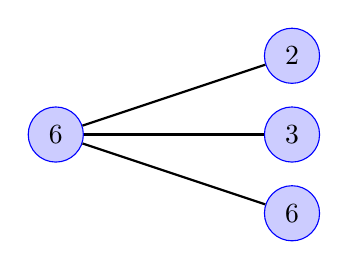
\begin{tikzpicture}[
						% Define a style for all nodes (optional, but helpful)
						node style/.style={circle, draw=blue, fill=blue!20, minimum size=7mm}
						]
						
						% Define and place your nodes
						\node[node style] (A) at (0, 0) {6};
						\node[node style] (B) at (3, 1) {2};
						\node[node style] (C) at (3, 0) {3};
						\node[node style] (D) at (3, -1) {6};
						
						% --- Draw the edges ---
						\draw[thick] (A) -- (B); 
						\draw[thick] (A) -- (C); 
						\draw[thick] (A) -- (D); 
					\end{tikzpicture}
					\vspace{12pt}
					\par %
					{Kenong nada 6 digunakan untuk me-ngenongi nada 2,3 dan 6}
				\end{center}
						
			\end{column}
			
		\end{columns}
		
	\end{frame}


	\begin{frame}
		\frametitle{Insight}
		\framesubtitle{Patet}
		Penggunaan kempyung memiliki relasi dengan patet.
		
		% Begin the columns environment
		\begin{columns}
			
			% --- First Column (Left Image) ---
			\begin{column}{0.5\textwidth}	
				\begin{center}
					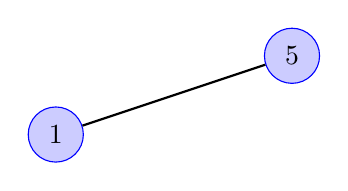
\begin{tikzpicture}[
						% Define a style for all nodes (optional, but helpful)
						node style/.style={circle, draw=blue, fill=blue!20, minimum size=7mm}
						]
						
						% Define and place your nodes
						\node[node style] (A) at (0, 0) {1};
						\node[node style] (B) at (3, 1) {5};
						
						% --- Draw the edges ---
						\draw[thick] (A) -- (B); 
					\end{tikzpicture}
					\par %
					\vspace{12pt}
					\textbf{Patet Sanga}
					\par %
					{Nada seleh 1 diberi kempyung 5}
				\end{center}
			\end{column}
			
			% --- Second Column (Right Image) ---
			\begin{column}{0.5\textwidth}
				\begin{center}
					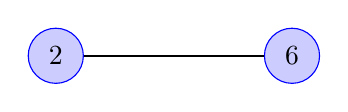
\begin{tikzpicture}[
						% Define a style for all nodes (optional, but helpful)
						node style/.style={circle, draw=blue, fill=blue!20, minimum size=7mm}
						]
						
						% Define and place your nodes
						\node[node style] (A) at (0, 0) {2};
						\node[node style] (B) at (3, 0) {6};
						
						% --- Draw the edges ---
						\draw[thick] (A) -- (B); 
					\end{tikzpicture}
				\par %
				\vspace{12pt}
				\textbf{Patet Nem dan Manyura}
				\par %
				{Nada kenong seleh 2 diberi kempul 6}
				\end{center}
			\end{column}
			
		\end{columns}
		
	\end{frame}


	
	\begin{frame}
		\frametitle{Insight}
		Martopangrawit menjelaskan bahwa dalam satu Gatra (unit 4 ketukan), terdapat distribusi berat/tekanan (stress).
		\begin{itemize}
			\item \textbf{Ketukan ke-4 (Sele/Seleh)}: Memiliki bobot paling berat (target nada/resolusi).
			
			\item \textbf{Ketukan ke-2}: Memiliki bobot berat (tapi tidak seberat ketukan ke-4). Sering disebut sebagai titik tumpuan tengah.
			
			\item \textbf{Ketukan 1 dan 3}: Memiliki bobot ringan (ketukan gantung).
			
		\end{itemize}
		\begin{figure}
			\centering
			\includegraphics[width=0.5 \linewidth]{maju-mundur-seleh.png}
		\end{figure}
		
		
	\end{frame}
	

	\begin{frame}
		\frametitle{Experimental Ideas}	% Begin the columns environment
		
		% 1. TOP ROW: TWO COLUMNS (50% each)
		\begin{columns}
			% --- Left Column (Row 1, Col 1) ---
			\begin{column}{0.48\textwidth}
				\centering
				\includegraphics[width=0.9\linewidth]{notasi-ayak-nem-slendro.png}
				\footnotesize{Notasi gamelan Ayak-ayakan Nem Slendro pt. Nem}
			\end{column}
			
			% --- Right Column (Row 1, Col 2) ---
			\begin{column}{0.48\textwidth}
				\centering
				\includegraphics[width=0.9\linewidth]{cmap-font-balungan.png}
				\footnotesize{Cmap font balungan.}
			\end{column}
		\end{columns}
		
		% Optional: Add a small vertical space between the rows
		\vspace{0.5em}
		\hrule % Optional: A horizontal line to visually separate the rows
		
		% 2. BOTTOM ROW: ONE MERGED COLUMN
		% We use \vfill to push the content to the bottom and a minipage to control its width
		\vfill 
		\begin{minipage}{\textwidth} % Minipage spans the full text width
			\centering
			
			\begin{figure}
				\centering
				\includegraphics[width=1 \linewidth]{notasi-ayak-nem-slendro-decoded.png}
				\caption{Notasi ayakan decoded}			
			\end{figure}
		\end{minipage}
		
	\end{frame}


	
	
	\begin{frame}
		\frametitle{Previous Work}
		\framesubtitle{Knowledge Representation}
		\begin{figure}
			\centering
			\includegraphics[width=1 \linewidth]{knowledge-representation-syarif.png}
			\caption{Representasi Knowledge Notasi untuk LSTM oleh Syarif (2023)}			
		\end{figure}
	\end{frame}
	
	\begin{frame}
		\frametitle{Previous Work}
		\framesubtitle{Knowledge Representation}
		\begin{figure}
			\centering
			\includegraphics[width=1 \linewidth]{knowledge-representation-lstm-fanani.png}
			\caption{Representasi Knowledge Notasi untuk LSTM and GA oleh Fanani (2025)}			
		\end{figure}
	\end{frame}
	\begin{frame}
		\frametitle{Rumusan Masalah}
		\framesubtitle{Cont..}
		\small Model LSTM pembangkit notasi gamelan yang dikembangkan oleh Syarif, A.M. dkk. (2023) memiliki keterbatasan pada aspek representasi data. \textbf{Notasi musik direpresentasikan deretan angka tanpa makna struktural}. Akibatnya, informasi penting mengenai bobot ketukan dalam Gatra (posisi seleh dan wilet) hilang. Model bekerja hanya berdasarkan probabilitas sekuens terdekat (lokal). Hal ini \textbf{menyebabkan kegagalan} model dalam menangkap dependensi struktural jangka panjang yang menjadi logika dasar musik gamelan.
		
		
	\end{frame}
	\begin{frame}
		\frametitle{Rumusan Masalah}
		\framesubtitle{Cont..}
		\small 
		
		Upaya mitigasi melalui pendekatan hibrida oleh Fanani, A.Z. dkk. (2025) mengandung \textbf{kontradiksi desain}. Algoritma Genetika (GA) digunakan tanpa operator crossover dengan premis bahwa output LSTM memiliki kualitas pola yang baik, namun secara paradoks menggunakan mekanisme mutasi intensif untuk menangani tingginya inakurasi. Tanpa crossover, GA terdegradasi menjadi pencarian acak yang tidak mewariskan fitur musikal unggul. \textbf{Akibatnya}, mekanisme validasi bekerja secara reaktif lokal. Sistem melakukan "tambal sulam" stokastik demi tercapainya validitas aturan dengan mengorbankan struktur melodis secara global.
		
	\end{frame}
	\begin{frame}
		\frametitle{Rumusan Masalah}
		\framesubtitle{Cont..}
		\small 
		
		Kombinasi keterbatasan tersebut menciptakan kesenjangan ilmiah yakni \textbf{belum tersedia model generatif yang mampu menyelaraskan kepatuhan aturan dan koherensi sekuensial dalam satu arsitektur terpadu}. Apabila tidak diatasi, model generatif akan terus memproduksi karya yang menyerupai gamelan namun cacat logika internal atau halusinasi algoritmik.
	\end{frame}

	\begin{frame}
		\frametitle{Mismatch Coherence Strategy}
			\begin{figure}
			\centering
			\includegraphics[width=0.7\linewidth]{pitch-mismatch.png}
			\caption{Contoh pitch mismatch method}			
		\end{figure}
	
	Fu X, Deng H, Yuan X, Hu J. Generating High Coherence Monophonic Music Using Monte-Carlo Tree Search. IEEE Trans Multimedia. 2023;25:3763–72. 
	\end{frame}

	\begin{frame}
		\frametitle{P.O.C}
		\begin{itemize}
			\item Bagana membuktikan incoherence?
			\item Reverese Paper :  LSTM, BiLSTM, G.A. Small prev dataset Gamelan
			\item Objective : Function untuk scoring tingkat coherence pada gamelan
		\end{itemize}
	\end{frame}
	
\end{document}
